%\documentclass[a4paper]{scrartcl}
\documentclass[a4paper]{article}
\usepackage{setspace}
\usepackage{url}
\usepackage{mdwlist}
\usepackage{polski}
\usepackage[utf8x]{inputenc}
\usepackage{color}
\usepackage{mathtools}
\usepackage{graphicx}
\usepackage[unicode=true]{hyperref}
\usepackage{multirow}
\usepackage[table]{xcolor}
\usepackage{subfig}
\usepackage{listings}
\usepackage[backgroundcolor=white]{todonotes}
\definecolor{dkgreen}{rgb}{0.2,0.8,0.2}
\definecolor{gray}{rgb}{0.5,0.5,0.5}
\definecolor{mauve}{rgb}{0.58,0,0.82}
\newcommand{\HRule}{\rule{\linewidth}{0.5mm}}
\newcommand{\siatkonator}{\textbf{Siatkonator XP} }
\renewcommand{\triangle}{\href{http://www.cs.cmu.edu/~quake/triangle.html}{triangle}}
\lstset{ %
  basicstyle=\ttfamily\footnotesize,
  numbers=left,
  numberstyle=\footnotesize,
  stepnumber=1,
  numbersep=5pt,
  breaklines=true,
  tabsize=2,
  showspaces=false,
  showstringspaces=false,
  frame=single,
  numberstyle=\tiny\color{gray},
  keywordstyle=\color{mauve},
  commentstyle=\color{dkgreen},
  stringstyle=\color{mauve},
}

\begin{document}
\begin{titlepage}

  \begin{center}


    % Upper part of the page
    
\includegraphics[width=0.3\textwidth]{logo.jpg}\\[1cm]

    \begin{onehalfspace}
      \textsc{\LARGE Wydział Elektryczny Politechniki Warszawskiej}\\[1.5cm]
    \end{onehalfspace}



    \textsc{Języki i~Metody Programowania II -- projekt 1}\\[0.5cm]

    % Title
    \HRule \\[0.4cm]
    {\huge \bfseries Siatkonator XP }\\[0.2cm]
    \HRule \\[1.5cm]

    % Author and supervisor
    \begin{flushleft} \large
      \emph{Autor:}\\
      Barnaba \textsc{Turek}\\
      \href{mailto:barnabaturek@gmail.com}{barnabaturek@gmail.com}
    \end{flushleft}
    \vfill

    % Bottom of the page
    {\large \today}

  \end{center}

\end{titlepage}
\sloppy

\setcounter{tocdepth}{4}
\tableofcontents

\section{Specyfikacja funkcjonalna}
\subsection{Program}
\siatkonator to program sklejający siatki trójkątne.
Program przyjmuje jedną lub więcej siatek trójkątnych oraz jeden wielokąt.
Wynikiem działania programu jest siatka trójkątna opisująca zadany wielokąt, która zawiera podane określone siatki.

Ponadto, program pozwala na wybór siatki i~otoczki przy użyciu graficznego interfejsu użytkownika. oraz wyświetla sklejoną siatkę.

Operacje na siatce dokonywane są za pomocą programu Siatkonator.

%\begin{figure}[h]
  %\centering
  %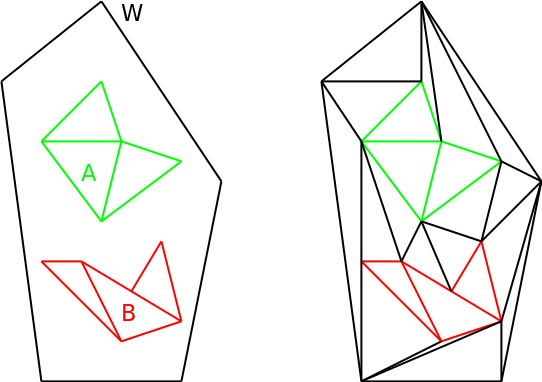
\includegraphics[width=0.5\textwidth]{ilustracja.png}
  %\caption{przykład sklejania zadanego wielokątu W~i~siatek A~i~B}
%\end{figure}

\subsection{Wywołanie}
Program nie przyjmuje argumentów linii poleceń.

\begin{lstlisting}[caption=Przykładowe wywołanie]
  $ siatkonatorXP
\end{lstlisting}

Program oferuje użytkownikowi dwie akcje, możliwe do wyboru po jego włączeniu:
\begin{itemize}
  \item Oglądanie wygenerowanych wcześniej plików \texttt{.node} i~\texttt{.ele} (ścieżka A).
  \item Sklejanie siatek z~otoczką (ścieżka B).
\end{itemize}

Zależnie od wybranej akcji wyświetlane ekrany są różne.

\subsection{Pliki}
\siatkonator korzysta z~plików w~formatach \texttt{poly}, \texttt{ele} i~\texttt{node}.

\begin{description}
  \item[poly] \href{http://www.cs.cmu.edu/~quake/triangle.poly.html}{format pliku opisującego wielokąt}
  \item[ele] \href{http://www.cs.cmu.edu/~quake/triangle.ele.html}{format pliku opisującego z~których wierzchołków składają się trójkąty siatki}
  \item[poly] \href{http://www.cs.cmu.edu/~quake/triangle.poly.html}{format pliku opisującego wierzchołki siatki}
\end{description}

Wszystkie wykorzystywane formaty są zgodne z~formatami wykorzystywanymi przez program \triangle.

\subsection{Projekt graficznego interfejsu użytkownika}
\subsubsection{Ścieżka wywołania A}
Jeśli użytkownik na ekranie numer \textbf{1} wybierze opcję ``Oglądaj .ele/.poly'', program zaprezentuje mu ekran \textbf{2A}, pozwalający wybrać plik .ele, który ma zostać wyświetlony.
Dostępna jest też opcja anulowania wyboru i~powrotu do ekranu \textbf{1}.

Na ekranie \textbf{2A} są wyświetlone tylko pliki \texttt{.ele}. Program zakłada, że istnieje plik o~rozszerzeniu \texttt{.node} i~tej samej nazwie bazowej, znajdujący się w~tym samym katalogu.

Kiedy użytkownik wybierze istniejący plik \texttt{.ele}, zostanie przeniesiony do ekran \textbf{4}, gdzie może obejrzeć siatkę.
Siatka jest automatcznie wycentrowana w~oknie, w~którym jest wyświetlana i~przeskalowana do takiego rozmiaru, żeby się w~nim mieściła.

Na ekranie \textbf{4}, możliwe jest też zapisanie plików \texttt{node} i~\texttt{ele} oraz powrót do menu głównego.

\subsubsection{Ścieżka wywołania B}
Jeśli użytkownik na ekranie numer \textbf{1} wybierze opcję ``Wybierz otoczkę'', program zaprezentuje mu ekran \textbf{2A}, pozwalający wybrać plik \texttt{.poly}, który ma zostać wyświetlony.
Dostępna jest też opcja anulowania wyboru i~powrotu do ekranu \textbf{1}.

Na ekranie \textbf{2B} są wyświetlone tylko pliki \texttt{.poly}.

Kiedy użytkownik wybierze istniejący plik \texttt{.poly}, zostanie przeniesiony do ekran \textbf{3B}, gdzie może obejrzeć otoczkę.
Po lewej stronie ekranu \textbf{3B} znajduje się pole, które pozwala na wybór katalogu (detal \texttt{1}).

Pod tym polem wyświetlone są znalezione w~katalogu siatki, przy każdej z~nich dostępny jest przycisk ``+'', który dodaje siatkę do listy siatek przeznaczonych do połączenia.

Poniżej znajduje się pole z~wybranymi siatkami, przy każdej znajduje się przycisk ``-'', pozwalający na usunięcie jednej z~siatek.
Wybrane siatki zostaną pokazane w~tym samym polu, co otoczka, jednak nie są sklejane od razu po dodaniu.

Ponadto na ekranie dostępny jest przycisk ``Generuj'', który spowoduje połączenie wybranych siatek z~otoczką.
Po wybraniu tej opcji użytkownik zostanie przeniesiony na ekran \textbf{4}, taki sam jak w~przypadku \emph{ścieżki wywołania A}.
Na ekranie widoczny będzie efekt sklejenia siatek z~otoczką.
Możliwe będzie zapisanie wygenerowanej siatki w~formacie plików \texttt{.ele} i~\texttt{.poly}.

\subsection{Komunikaty błędów}
Program w~razie napotkania błędu wyświetla okienko z~krótkim komunikatem. Dostępne są następujące komunikaty:

\begin{itemize}
  \item ``Nie można odczytać pliku''
  \item ``Błąd w~formacie pliku''
  \item ``Błąd w~komunikacji z~procesem Siatkonator''
  \item ``Funkcjonalność nie zaimplementowana''
\end{itemize}

\end{document}
